\documentclass[12pt]{article}

% Packages
\usepackage[letterpaper, margin=1in]{geometry}
\usepackage{enumitem}
\usepackage{titlesec}
\usepackage{xcolor}
\usepackage{graphicx}
\usepackage{siunitx}
\usepackage{upgreek}
\usepackage{natbib}
\usepackage{xspace}
\usepackage{longtable}
\usepackage{multirow}
\usepackage{mdframed}
\usepackage{minted}
\usepackage{lipsum}
\usepackage[acronym]{glossaries}
\usepackage[
  colorlinks=true,         % enable colored links
  linkcolor=blue,          % color of internal links
  citecolor=green,         % color of links to bibliography
  filecolor=magenta,       % color of file links
  urlcolor=cyan            % color of external links
]{hyperref}

\hypersetup{
    citecolor=blue
}


% Document Settings
\usepackage{parskip} % Adds spacing between paragraphs
\setlength{\parindent}{0pt} % Removes first-line indent from paragraphs

% command
\newcommand{\museismic}{$\upmu$seismic\xspace}
\newcommand{\muquake}{$\upmu$Quake\xspace}

\DeclareSIUnit{\foot}{ft}

\makeglossaries
% \setabbreviationstyle[abbreviation]{long-short}


\newacronym{das}{DAS}{distributed acoustic sensing}
\newacronym{ai}{AI}{artificial intelligence}
\newacronym{fba}{FBA}{force balance accelerometer}
\newacronym{hdf5}{HDF5}{hierarchical data format version 5}
\newacronym{asdf}{ASDF}{adaptable seismic data format}
\newacronym{seed}{SEED}{standard for the exchange of earthquake data}
\newacronym{utc}{UTC}{coordinated universal time}
\newacronym{nrl}{NRL}{nominal response library}
\newacronym{smti}{SMTI}{seismic moment tensor inversion}
\newacronym{ppv}{PPV}{peak particle velocity}
\newacronym{ppa}{PPA}{peak particle acceleration}
\newacronym{ned}{NED}{north east down}
\newacronym{enu}{ENU}{east north up}






\begin{document}
\title{$\upmu$Seismic Data Exchange Format for in-Mines System (MDEFM) - RFC}
\author{Jean-Philippe Mercier}
\date{\today}
\maketitle

\newpage
\section*{Executive Summary}
\addcontentsline{toc}{section}{Executive Summary} % Optional: to include in TOC

\lipsum[1-2] % Replace with your summary text

\newpage

\tableofcontents
\pagebreak

\section{Introduction}
\subsection{Purpose}

This RFC aims to invite comments on a suggested format to allow for standardized and consistent access to \museismic data collected by mine \museismic monitoring systems. The proposed conventions and format objective is to enable a seamless, lossless and convenient exchange between different platforms. It considers future needs for developing high-performance, flexible, and accurate artificial intelligence that is envisioned to use the full range of available seismic data. 

Note that the objective of the proposed standard \textbf{does not} concern or prescribe how seismic data are \textbf{internally managed} within proprietary platforms, although the proposed implementation is designed for high performance and computational efficiency and would be suited for that purpose.

The proposed standard applies to triggered events and continuous recording alike and is suited for efficiently storing the high-density \gls{das} data.

Access to the \museismic data collected by in-mine monitoring systems is currently inconsistent. Variations arise from site to site and vendor to vendor and are often tailored to third-party requests. Such inconsistencies lead to inefficiencies, making data usage unnecessarily challenging and limiting the potential of \museismic data.

To ensure mines have access to technologies and approaches leading to optimal outcomes permitting the safe and productive operation of mines, allowing unrestricted access to \museismic data in a standardized format is a must. 

This document proposes conventions and a format for the lossless and seamless exchange of \museismic data. 

We seek alignment from different stakeholders, including \museismic system and service providers, end-clients, industry practitioners, academic researchers, and research institutions.

\subsection{Scope}

The standard outlined in this RFC seeks to:

\begin{itemize}
    \item Define comprehensive data formats and structure for \museismic data exchange, encapsulating all necessary data elements and fostering the normalization of data processing and analysis. The proposed framework is designed to enhance interoperability between various sites and vendors, minimizing discrepancies stemming from the lack of common reference.
    \item Define mechanisms to extract partial topical information conveniently (e.g., a standard CSV representation of catalog data).
    \item propose adaptations to the base format to capture the essence of mining data.
    \begin{itemize}
        \item defining a list of acceptable event types in mining.
        \item establishing an unequivocal and standardized naming convention for the logical organization of the seismic system components.
        \item prescribing a directory structure and file naming convention.
    \end{itemize}
\end{itemize} 

\subsection{Objective}

This RFC aims to:

\begin{itemize}
    \item Foster a standardized representation of \museismic data, creating a universally accepted convention and eliminating fragmented or inconsistent data representations.
    \item Facilitate an efficient mechanism for the storage, dissemination, and accessibility of \museismic data. Ensuring versatility and catering to diverse applications ranging from real-time processing to long-term data analysis.
    \item Promote cross-platform compatibility, ensuring the data can be seamlessly processed, interpreted, and utilized irrespective of the platform, tool, or system.
    \item Enhance data integrity, ensuring it remains consistent, accurate, and unaltered during exchanges, making it reliable for various analytical and operational purposes.
\end{itemize}

\subsection{Rationale}

\subsubsection{Need for a New Standard}

The increase in microseismic data, particularly from expansive monitoring systems and new technologies like \gls{das}, underscores the pressing need for an efficient and unified data format. Currently, the system information, catalog and waveform data are provided in a series of file that does not allow simple cross-referencing. For instance, one file may refer to a sensor with a long name, whereas another uses a numerical ID. The link between the name and the numerical ID is left ambiguous. Some other essential information such as the sensor types to identify whether the sensor is a \SI{4.5}{\hertz} or \SI{15}{\hertz} geophone, a high-frequency accelerometer or a low-frequency \gls{fba}. 

The varied nature of microseismic data formats hinders streamlined integration and analysis, posing challenges in managing and deriving value in datasets collected by in-mine monitoring systems. The lossy and incoherent nature of current data exchange formats hinders innovation and makes the utilization of \museismic data unnecessarily tricky. Given the critical importance of microseismic data in ensuring safety and improving underground mining operations, establishing a standardized format and mechanism of exchange becomes imperative. The proposed standard objective is facilitating more straightforward data access, efficient storage, smoother data exchanges across different platforms, and accommodating various data types.



\section{Terminology and Definitions}
\begin{description}
    \item[Waveforms] -- A time series representation of seismic wave amplitudes detected by sensors in microseismic monitoring. Originating from subsurface events like rock fractures.
    \item[Catalog/Seismic Bulletin] -- A curated collection of detected and processed microseismic events, systematically listing key parameters such as event origin time, location, magnitude, corner frequency, and energy. Derived from waveform analysis, the catalog serves as a comprehensive record of seismicity.
    \item[Inventory] -- A structured repository detailing the metadata of seismic networks, stations, and their associated instrumentation. It encompasses station location, operational time periods, instrument response, and channel configurations.
    \item[SEED] -- A standardized format for representing and exchanging digital seismological data encompassing waveform records and related metadata. Established by the Federation of Digital Seismographic Networks (FDSN), SEED (Standard for the Exchange of Earthquake Data) is widely adopted for its ability to consolidate seismic data and its associated station and instrument information into a unified structure, ensuring consistency and interoperability in seismological research and monitoring.
    \item[MiniSEED] -- A subset of the SEED format specifically designed for the exchange and storage of seismic waveform data. While the broader SEED standard encompasses data and comprehensive metadata, MiniSEED focuses solely on time series data, making it more compact and suitable for efficient data transmission and storage. Despite its simplicity, MiniSEED retains the essential headers for data identification and integrity, ensuring its applicability in diverse seismological applications.
    \item[QuakeML \citep{quakeml}] -- A standardized XML-based data format developed for representing and exchanging seismological data related to earthquakes. By covering event parameters like origins, magnitudes, and phase picks, QuakeML aims to facilitate interoperability and consistency in sharing and processing seismic event information across various seismological tools and platforms. Its structured schema ensures that earthquake-related data are described comprehensively yet flexibly, catering to diverse seismological research and monitoring needs.
    \item[StationXML \citep{stationxml}] -- A modern XML-based format designed for the representation and exchange of metadata associated with seismic stations, networks, and associated instruments. Evolved as a successor to the SEED format's metadata component, StationXML provides a detailed description of station configurations, instrument response information, and operational time periods, among other attributes. Its structured framework ensures a comprehensive and consistent portrayal of the seismic data acquisition chain, promoting accurate data interpretation and seamless exchange across seismological applications.
    \item[HDF5 (Hierarchical Data Format version 5)] -- An advanced data model, library, and file format designed for storing and organizing large volumes of complex data, including arrays of numbers, multidimensional datasets, and metadata. \gls{hdf5} is optimized for high performance and flexibility, allowing for efficient storage and retrieval across diverse platforms and languages. Its hierarchical structure supports grouping related objects and tagging with rich metadata, making it a widely adopted choice for scientific computing applications where complex datasets and their associated metadata need to be integrated.
    \item[ASDF (Adaptable Seismic Data Format)] -- A modern data format explicitly designed for seismological data and related metadata. Building on the \gls{hdf5} infrastructure, \gls{asdf} is tailored for efficiency, scalability, and adaptability in both storage and processing of seismic data. It facilitates the integration of raw waveforms, processed data products, event parameters, and station metadata within a single file structure. The format's adaptability and hierarchical structure ensure consistent and optimized handling of diverse seismic datasets, making it a valuable choice for advanced seismological research and applications.
    \item[Sensor] -- A device specifically designed to detect or measure a physical property and convert this input into an electrical signal. A sensor (e.g., geophone element) is responsible for directly detecting seismic waves and transducing them into voltage variations based on its sensitivity. Example: a \SI{4.5}{\hertz} geophone
    \item[Instrument] -- A comprehensive setup encompassing one or multiple sensors and associated components, including casings, and internal electronics if applicable. In microseismic monitoring, an instrument refers to the entire arrangement employed for seismic detection. Its response combines the characteristics of the individual sensors. Example: a tri-axial dual element geophone.
    
\end{description}

\section{General Format Considerations}
\subsection{General Format Considerations}

This section delves into the overarching design principles and foundational elements underpinning the proposed format, ensuring adherence to the objectives of seamless, lossless, and convenient data interchange across platforms.

\begin{enumerate}
    \item \textbf{Data Integrity and Consistency}: Details on mechanisms, potentially including checksums, versioning, or other measures, to ensure data remains unaltered and consistent during transfers.
    
    \item \textbf{Platform Independence}: Insights into how the format maintains neutrality to specific proprietary platforms, endorsing cross-platform compatibility.
    
    \item \textbf{Scalability and Flexibility}: Addressing the format's ability to manage both small and expansive datasets, e.g., high-density \gls{das} data.
    
    \item \textbf{Usability}: Features enhancing the user-friendliness of the format, which may encompass aspects like readability, annotations, or metadata.
    
    \item \textbf{Efficiency}: Discussion around computational considerations, ensuring both data storage and exchange remain efficient.
    
    \item \textbf{Extensibility}: Considerations on the format's design, allowing it to evolve and accommodate future technological shifts or data needs.
    
    \item \textbf{Standardized References}: Incorporating standardized naming conventions, directory structures, and file naming conventions.
    
    \item \textbf{Interoperability with Existing Formats}: Examination of the format's relationship or interaction with prevailing data formats in the domain.
\end{enumerate}


\section{Essential Data Exchange Content}
% The data requirements are closely correlated with the intended purpose. For some applications, the delivery of catalog data alone may be sufficient, that is, if the data quality is high enough and one is confident enough in the classification, location and source parameters. For other applications, having access to the waveform is a must. For instance, applications based on artificial intelligence and machine learning greatly benefit from direct access to the waveforms and all the information required to make sense of the data. Information from the catalog can be used as parameters, but are often not optimal and lead to ill-posed problems where the model space does not afford the level of orthogonality permitting an unambiguous solution. Exploiting the waveforms requires having access to the inventory or system information. This type of metadata allows for the localization of the acquisition instrument and provides information on the sensor's nature and response. Another important metadata that is often overlooked, is the velocities. For more and more applications, it is difficult to make sense of the information or reproduce the data without knowledge of the underlying velocity models. It is becoming increasingly frequent for 3D velocity grids to be utilized in the processing of the data. 

\subsection{overview}

The intended application directly governs the specificity of data requirements. When catalog data meets quality standards and its classification, location, and source parameters are reliable, it may suffice for certain applications. However, for more demanding or complex tasks, raw waveforms and accompanying metadata become essential. Sole reliance on catalog data in such instances often leads to ill-posed problems characterized by insufficient model space orthogonality and ambiguous solutions. To fully leverage waveform data, access to inventory or system metadata is imperative for instrument localization and sensor characterization. For completeness, one could also benefit from access to seismic velocities, especially when 3D models are used.

\section{Seismic System Information Categories}

Seismic system information can be partitioned into four main categories:

\begin{description}
    \item[Catalog] Catalog data includes processed attributes related to seismic events: time, location, magnitude, amplitude (\gls{ppv}, \gls{ppa}), classification, \textit{P}- and \textit{S}-wave picks, and moment tensor/focal mechanism data.
    
    \item[Inventory] Details the seismic network, stations, and sensor configurations. This includes sensor location, type, response, and orientations. Inventory data should facilitate necessary data manipulation for analysis.
    
    \item[Waveform] Raw or event-triggered time-series data recorded by the instruments, foundational for all seismic analyses.
    
    \item[Velocities/Travel Time Grids] Required for location, magnitude calculation, and moment tensor inversion. Allows for ray tracing and wavefield rotation to isolate \textit{P}- and \textit{S}-waves.
\end{description}

Information in these categories must be internally coherent, enabling straightforward cross-referencing and understanding of data provenance and relationships.

\subsection{Waveforms}

Waveforms should include:

\begin{itemize}
    \item Instrument and channel ID
    \item Sampling rate or interval
    \item Start time
    \item Amplitude, in ADC counts or physical units
\end{itemize}

\subsection{Catalog}

Catalog data is bifurcated into:

\begin{description}
    \item[Event-related] Minimum requirements:
    \begin{itemize}
        \item Time (local and UTC)
        \item Location
        \item Classification 
        \item Magnitude, along with seismic moment \( M_0 \) and corner frequency \( f_c \) for moment magnitude
        \item Radiated energy for \textit{P}- and \textit{S}-waves
        \item Moment tensor solution if available
    \end{itemize}
    \item[Waveform-related] Derived from waveform data:
    \begin{itemize}
        \item Picks: \textit{P}- and \textit{S}-wave onset times
        \item Amplitude: Information, evaluation mode, and status
    \end{itemize}
\end{description}

\subsection{Inventory}

Minimum inventory requirements:

\begin{itemize}
    \item Instrument ID
    \item Location
    \item Channel orientations
    \item Instrument response, per channel
\end{itemize}

\subsection{Velocity Grids}

A functional velocity grid should comprise:

\begin{itemize}
    \item Origin
    \item Spacing between grid nodes
    \item Dimensions: Number of grid points in each axis
    \item Data: Grid values
    \item Units (\si{\meter} or \si{\foot})
\end{itemize}








\section{Data Format for Seismic Data}
\subsection{Overview}

The recommended seismic data standard for adoption is the \glsdesc{asdf} (\gls{asdf}) \citep{krischer2016asdf}. Designed with modern challenges in mind, the \gls{asdf} format efficiently addresses the complexities inherent to large and detailed seismic datasets. By employing the HDF5 container format, \gls{asdf} is self-descriptive, ensuring data can be accessed and manipulated with ease across various seismological applications. Its overarching objective is to simplify the organization and exchange of seismic data, emphasizing interoperability, scalability, and the reduction of inconsistencies by amalgamating multiple seismic data components within a singular structure. The \gls{asdf} format is suitable for trigger, continuous and \gls{das} data to name only those.

Figure~\ref{fig:asdf_data_format} depicts the structure of the \gls{asdf} format. Nested within the \glsdesc{hdf5} (\gls{hdf5}) container, \gls{asdf} systematically organizes seismological components, including:

\begin{description}
    \item[uakeML] An XML-based language, QuakeML focuses on event metadata, cataloging seismic event descriptions such as event origins, magnitudes, and moment tensor solutions.
    
    \item[Waveform Data] The heart of the \gls{asdf}, this section contains time series representations of seismic waveforms. In the \gls{asdf} format, waveform data are exclusively represented using single and double precision floating point values, or signed integers. These representations are encapsulated as native data arrays within the HDF5 framework.

    \item[StationXML]: Serving as a repository for station metadata, this section contains detailed instrument information, including their responses, station coordinates, and other specific attributes. This metadata provides vital context to the waveforms. In the \gls{asdf} format, this inventory information is appended directly to the waveforms at the station level.
    
    \item[Auxiliary Data]: Catering to the diverse needs of seismological analyses, this section allows storage of additional data types, such as cross-correlations or synthetic seismograms.
    
    \item[Provenance Data]: In the pursuit of rigorous transparency and reproducibility, this segment meticulously documents the historical progression of data alterations, enumerating each distinct processing operation along with its respective parameters. The provenance documentation adheres to the W3C PROV model \citep{w3cprov2013}, a widely accepted standard for chronicling provenance specifics.

\end{description}

\begin{figure}
    \centering
    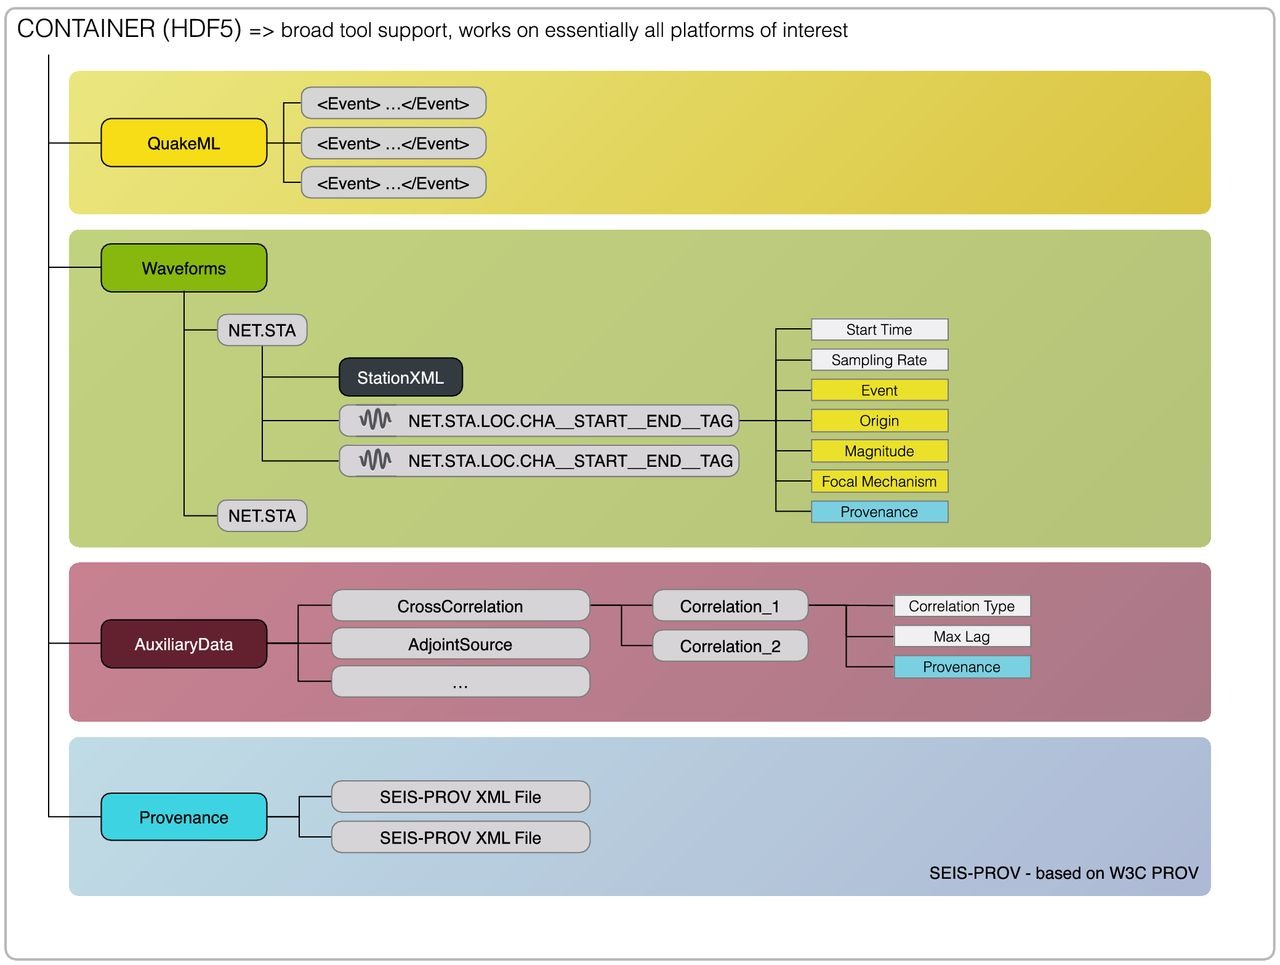
\includegraphics[width=\textwidth]{ASDF_Format_overview.jpeg}
    \caption{\gls{asdf} data structure overview from \citet{krischer2016asdf}}
    \label{fig:asdf_data_format}
\end{figure}

Through its comprehensive integration of these components, \gls{asdf} paves the way for a standardized, efficient, and in-depth approach to seismological research and data management.

While the \gls{asdf} format provides a robust framework for general seismic data handling, specific adaptations are imperative to address the unique requirements of \museismic monitoring within mining environments. Notably, the inherent geographical coordinate system utilized in \gls{asdf}, based on latitude and longitude, necessitates transformation to a Cartesian coordinate system (x, y, z) to represent in-mine locations accurately. These conversions are essential for precise data representation and effective integration with other mining systems. The proposed changes are not fundamentally altering the \gls{asdf} standard. Instead, they leverage the inherent flexibility and expandability of the QuakeML and StationXML formats, ensuring that the adapted schema remains consistent with the broader seismological community's practices.

\begin{mdframed}[backgroundcolor=gray!20]
\textbf{Note on Coordinate Systems:} Utilizing a Cartesian coordinate system (x, y, z) introduces inherent ambiguities. Notably, the orientation of the x and y axes could align either with the North and East directions or be reversed. Additionally, the direction of the z-axis could be either upwards or downwards. To mitigate these ambiguities, we recommend imposing constraints on the alignment of the x, y, and z axes to ensure the coordinate system is right-handed and aligned with geographical axes. Specifically, we advocate the use of \gls{enu} and \gls{ned} coordinate systems.

\muquake version 2.2.0 introduces the \texttt{Coordinates} Class and implements the management of the Cartesian coordinate system in the relevant Obspy objects, allowing the integration of the information in the QuakeML and StationXML format (see Appendix~\ref{app:coordinate_system_handling}). The handling is done by converting the \texttt{Coordinate} object to JSON and writing the JSON string as an extra parameter in the relevant sections.
\end{mdframed}

Note that the modifications discussed in the following sections, particularly concerning QuakeML and StationXML formats, have been operationalized in the \muquake library. This library extends the Obspy package and is tailored to the specific needs of \museismic monitoring within the mining contexts. Code examples detailing these customizations in \muquake will be provided later in the document, demonstrating how these adaptations can be seamlessly integrated into existing data manipulation workflows.


The most significant deviation from the Obspy object definition concern the 


\subsection{QuakeML}
\subsubsection{Modifications}

\begin{table}[!h]
\centering
\caption{Summary of Modifications}
\begin{tabular}{lllr}
\hline
\textbf{Object} & \textbf{New Parameter} & \textbf{Description} & \textbf{Type} \\
\hline
\multirow{1}{*}{Origin}     & Coordinates & Coordinates information & Coordinates\footnote{Coordinate class described in the Appendix~\ref{app:coordinate_system_handling}} \\
\hline
\multirow{3}{*}{Magnitude}  & \(f_0\) & Corner frequency & float \\
                            & \(E_p\) & \(P\)-wave energy & float \\
                            & \(E_s\) & \(S\)-wave energy & float \\
\hline
\end{tabular}
\end{table}

We propose straightforward modifications to the QuakeML format to better suit \museismic applications. The first concerns the expression of coordinates using the Cartesian system previously described instead of the longitude, latitude, and depth/elevation. The second pertains to expanding the magnitude definition to include the corner frequency and the \textit{P}- and \textit{S}-wave velocities. The third involves the overriding of event types.

Instead of the standard spherical coordinate system that relies on latitude and longitude for location specification, we advocate for a Cartesian coordinate system. Specifically, we recommend emptying the traditional fields for latitude, longitude, elevation, and depth. As a substitute, we propose adding a description of the Coordinates as a new field. The coordinate description object is implemented in \muquake from version 2.2.0. In the current implementation, the information is stored as a JSON string in the extra parameters of the Origin description of the  QuakeML file. The coordinate object includes the x, y, and z coordinate, a description of the coordinate system (either \gls{enu} or \gls{ned}), and elements to allow for converting the coordinates between multiple representations including latitude, longitude if the required information is provided.

We propose an enhancement to the magnitude definition in QuakeML to represent seismic source properties better. The existing schema falls short in capturing key parameters such as the corner frequency ($f_0$), and the \textit{P}- and \textit{S}-wave energies ($E_p$ and $E_s$, respectively). Similar to our approach for coordinate system modification, we suggest including $f_0$, $E_p$, and $E_s$ in the extra parameters section of the QuakeML schema. This enables the on-the-fly calculation of other source parameters using the seismic moment ($M_0$), corner frequency, and wave energies. Relationships among these source parameters are elaborated in Appendix~\ref{sec:app_source_params}.

Transitioning to event classifications, the QuakeML schema has a predefined set of seismic event types that do not fully accommodate the specialized needs of \museismic monitoring. We propose mapping existing event types to new, mining-specific descriptors and directly including a generic look-up table in the code for on-the-fly translation. While efforts were made to create logical mappings, limitations in the existing event types posed challenges in finding intuitive counterparts. Table~\ref{tab:event_type_mapping} presents this mapping between standard and \museismic event types.

\begin{longtable}{ll}
    \caption{Mapping between standard and \museismic event types.} \label{tab:event_type_mapping} \\
    \hline
    Event Type (mining) & Event Type (QuakeML) \\
    \hline
    \endfirsthead
    \multicolumn{2}{c}%
    {{\bfseries \tablename\ \thetable{} -- continued from previous page}} \\
    \hline
    Event Type (mining) & Event Type (QuakeML) \\
    \hline
    \endhead
    \hline 
    \multicolumn{2}{r}{{Continued on next page}} \\
    \endfoot
    \hline
    \endlastfoot
    earthquake/large event & earthquake \\
    seismic event & induced or triggered event \\
    offsite event & atmospheric event \\
    rock burst & rock burst \\
    fall of ground/rockfall & cavity collapse \\
    blast & explosion \\
    blast sequence & accidental explosion \\
    development blast & industrial explosion \\
    production blast & mining explosion \\
    far away blast/open pit blast & quarry blast \\
    offsite blast & nuclear explosion \\
    paste firing & chemical explosion \\
    calibration blast & controlled explosion \\
    other blast/slashing & experimental explosion \\
    mid-shift blast/slash blast & industrial explosion \\
    raise bore & hydroacoustic event \\
    crusher noise & road cut \\
    orepass noise & collapse \\
    drilling noise & acoustic noise \\
    electrical noise & thunder \\
    scaling noise & anthropogenic event \\
    mechanical noise & crash \\
    test pulse & sonic boom \\
    unidentified noise/other noise & other event \\
    duplicate & boat crash \\
    unknown & plane crash \\
    tap test/test & avalanche \\
\end{longtable}

\paragraph{Parameter Validation}
The validation for the newly introduced parameters is performed within the \muquake library. For standard parameters, validation is handled by the Obspy package. This ensures a cohesive framework for both standard and specialized seismic data types.


\subsection{Waveforms and StationXML}

\subsubsection{Modifications}

\begin{table}[!h]
\centering
\caption{Summary Modifications}
\begin{tabular}{lllr}
\hline
\textbf{Object} & \textbf{New Parameter} & \textbf{Description} & \textbf{Type} \\
\hline
\multirow{1}{*}{Network} & Time Zone & IANA Time Zone or time offset & string \\
\hline
\multirow{3}{*}{Station} & x & x-coordinate & float \\
                         & y & y-coordinate & float \\
                         & z & z-coordinate & float \\
\hline
\multirow{5}{*}{Channel} & x & x-coordinate & float \\
                         & y & y-coordinate & float \\
                         & z & z-coordinate & float \\
                         & oriented & True if orientation is known & boolean \\
                         & active & True if the channel is active & boolean \\
\hline
\end{tabular}
\end{table}

In a manner analogous to our QuakeML modifications, we adapt the StationXML format to meet the specific needs of the \museismic context. The changes affect the \texttt{Network}, \texttt{Station}, and \texttt{Channel} definitions. Support for a local coordinate system is added to the \texttt{Station} and \texttt{Channel} definitions, and two new parameters are introduced in the \texttt{Channel} definition to indicate orientation and current activity status. The mutable 'active' flag allows for the temporary exclusion of a component due to timing issues or other transient problems. These changes, include support of the \texttt{Coordinates} object in the \texttt{Station} and \texttt{Channel} objects, and the storage of the \texttt{Coordinates} as JSON string in the extra parameters section. Time zone information is added to the Network definition to facilitate conversion between local and UTC time. The provided time zone must either represent an offset from Coordinated Universal Time (UTC) or correspond to a valid entry in the \href{https://www.iana.org/time-zones}{IANA time zone database}. The \muquake library ensures seamless integration of these modifications and replicates Obspy's default behavior regarding location data. It also allows the extraction of predefined values from the extra parameters section as typical object properties.

The waveform format does not require any alteration.

\paragraph{Parameter Validation}
As for the QuakeML, the validation for the newly introduced parameters is performed within the \muquake library. For standard parameters, validation is handled by the Obspy package. This ensures a cohesive framework for both standard and specialized seismic data types.

\subsubsection{Stream Naming Convention}

The \gls{asdf} file format combines waveforms and inventory data. To ensure flawless integration, we must adopt a robust and standardized "stream" naming convention to ensure unambiguous association between waveforms and inventory. 

\gls{asdf} adopts a relaxed version of the \gls{seed} Identifier Convention previously part of QuakeML and StationXML standards and now extended to the waveform data. The StationXML does not restrict the string length; QuakeML does. We therefore suggest adopting the convention presented in section 3.3.5 of the QuakeML Version 1.2 (revision 20130214b) (see \href{https://quake.ethz.ch/quakeml/docs/latest?action=AttachFile&do=get&target=QuakeML-BED.pdf}{QuakeML Reference Manual}). This convention provides a standardized approach to uniquely identify seismic data streams by anchoring them to their source network, station, location, and channel, ensuring clarity and consistency in data identification and handling across various seismic data systems.

The QuakeML naming convention comprises four distinct parts that are:

\begin{description}
  \item[Network] Represents a collection of stations grouped by a specific monitoring objective or designed to target a distinct area within a mine. This grouping may not necessarily reflect physical proximity but is often organized based on monitoring needs or operational considerations.
  \item[Station] Within a given network, the term station denotes a coordinated set of instruments, often clustered together based on their monitoring function or spatial considerations. For example, a station can comprise a set of instruments installed in a single borehole or deployed from the same location in boreholes of different orientations.
  \item[Location] Specifies an individual instrument within a station, allowing differentiation when multiple instruments exist at the same station. For example, each instrument would refer to a location in a borehole where multiple instruments are installed.
  \item[Channel] Details the specific recording component or the type of measurement undertaken by the instrument at the given location.
\end{description}

A unique stream name is obtained by concatenating those parts together as follows:
\begin{center}
\texttt{NETWORK.STATION.LOCATION.CHANNEL}
\end{center}

\subsubsection{Waveform Representation and Response Correction}

Waveform data in \museismic can be stored as either integers representing ADC counts or as physical units such as \si{\meter}, \si{\meter\per\second}, and \si{\meter\per\second\squared} using 32-bit single-precision floats. An essential aspect of data integrity and interpretation is the correction of the instrument's response, embedded in the StationXML. The \muquake library, through Obspy, provides functionalities for both response correction and unit transformation, allowing the waveforms to be accurately expressed in terms of acceleration, velocity, or displacement. Detailed guidelines for constructing the instrument's response and examples for correction are discussed in Appendix~\ref{sec:app_response}.

 
\subsection{Auxiliary Data}

\subsubsection{Overview}

The design of the ASDF format incorporates provisions for extensibility, enabling the inclusion of auxiliary data beyond the predefined schema for catalogs, inventory information, and waveform data. Given the dynamic and varied nature of seismological research, and the specificity of the different fields where seismology applies, including \museismic monitoring in mines, it is neither possible nor practically feasible to create a rigid schema that accommodates all potential use cases. While ASDF prescribes a structured format for fundamental seismic data types like catalogs, inventory, and waveforms, it concurrently provides flexible containers which structure is yet to be defined. These containers capture the broad and evolving range of applications in seismology, both current and future, thereby ensuring the format's utility and relevance over time.

Auxiliary data in ASDF is intentionally loosely defined, allowing for a broad range of data types beyond seismic waveforms. Each piece of auxiliary data is allocated within an arbitrarily nested path in the auxiliary data group. The data can take on any dimensional form, accompanied by a flexible key-value representation for metadata. This flexibility is not accidental but rather designed to cater to the rapidly evolving needs and active research in various areas of seismology.

As of version 2.0, \muquake offers support for the ASDF format, although it has yet to exploit the format's full capabilities. To date, \muquake has implemented methods to store two types of auxiliary data that enhance the system performance: rays and alternative event locations obtained through resampling methods used for statistical uncertainty estimation, including Monte Carlo and jackknife techniques. These inclusions obviate the need for repeated, computationally intensive operations by saving results for future use. Looking ahead, we anticipate that community-driven conventions for storing other types of data will emerge, further leveraging the extensibility of the ASDF format for standardized and comprehensive data storage.


\subsubsection{Rays}

Rays and their derivative information serve as key inputs in microseismic monitoring analyses, such as magnitude calculation and \gls{smti} evaluation. Calculating these rays on the fly poses computational challenges. Without precomputed rays, analyses often resort to the straight-ray assumption or require resource-intensive recalculations. Microseismic monitoring systems rarely keep or save ray information due to the lack of containers or structures for preserving it. This hinders the ability to easily reproduce results, especially when velocity models and travel-time grids are not readily accessible. Storing rays in the ASDF file within \muquake streamlines computational processes by obviating repetitive, costly ray tracing and by providing more complete information downstream.

\begin{table}[!h]
\centering
\caption{Ray Object Data Structure}
\begin{tabular}{|l|l|p{6cm}|l|}
\hline
\textbf{Object} & \textbf{Parameter} & \textbf{Description} & \textbf{Type} \\
\hline
\multirow{4}{4cm}{WaveformStreamID} & site\_code & Site code of the receiver station & str \\
                                    & event\_id & ResourceIdentifier for the seismic event & ResourceIdentifier \\
                                    & origin\_id & ResourceIdentifier for the origin & ResourceIdentifier \\
                                    & arrival\_id & ResourceIdentifier for the arrival & ResourceIdentifier \\
\hline
Ray trace & nodes & List of 3D coordinates defining the ray path & np.array \\
\hline
Ray parameters & phase & Seismic phase (P or S) & str \\
               & azimuth & Azimuth angle in degrees & float \\
               & takeoff\_angle & Takeoff angle in degrees & float \\
               & travel\_time & Travel time in seconds & float \\
\hline
Metadata & earth\_model\_id & ResourceIdentifier for the Earth velocity model & ResourceIdentifier \\
\hline
\end{tabular}
\end{table}








\subsubsection{Uncertainty Cloud}


rays, alternative locations, system information.





\section{Data Format for Grids}
\subsection{overview}

The HDF5 format is a flexible, high-performance data storage format designed for complex, large datasets. In the context of storing grid information, HDF5 offers a hierarchical file structure similar to a file system, facilitating the organization of data into groups and datasets. This structure allows for efficient and intuitive storage of multidimensional grid data, along with associated metadata, in a single, portable file.

We suggest defining two types of grids: 
\begin{description}
    \item[Global] Grids that apply to the entire network like the \textit{P}- and \textit{S}-wave velocities grids
    \item[Instrument Specific] Grids that apply to a specific instrument, like the travel time and angle grids
\end{description}

For the purpose of microseismic monitoring, we suggest organizing the information by storing all similar elements in a single file. For example, we would store all the velocity models in one file, all the travel time grids in another and the angle grids in yet another. 

In this context, we suggest limiting the scope of the grid storage to two types of structured grids: regular or rectilinear grids. 

\begin{description}
    \item[Regular Grid] A grid in which the spacing between the points is constant in each dimension. In 3D, this would resemble a cubic lattice.

    \item[Rectilinear Grid] A grid in which the spacing between the points can vary along each axis but remains orthogonal. In 3D, this would look like a deformed cubic lattice where the deformations are axis-aligned.
\end{description}

Note that the regular grid is a special case of a rectilinear grid where the spacing is the same along each axis. 

\subsubsection{General Format}

The grid data structure, whether global or instrument-specific, contains common elements that define its geometry and facilitate its interpretation. A straightforward yet effective description can be achieved using the origin, spacing, and dimensions of the grid.

\begin{description}
    \item[Origin] The origin refers to the coordinate point in the grid where the spatial indices are (0,0,0). It acts as the reference point for other grid points and is specified in the coordinate system used (e.g., ENU or NED).
    
    \item[Spacing] The spacing describes the distance between adjacent grid points along each axis (x, y, z). It dictates the resolution of the grid. In regular grids, the spacing is constant, while in rectilinear grids, it can vary along each axis. The spacing is generally provided in units consistent with the chosen coordinate system.
    
    \item[Dimensions] The dimensions specify the total number of grid points along each axis (x, y, z), thereby determining the overall size and shape of the grid.
\end{description}


\subsection{Global Grids}

To take advantage of the hierarchical nature of the HDF5 file format, we suggest storing the global grids, which includes the velocity grids, 

\begin{tabular}{|l|l|l|}
\hline
\textbf{Field} & \textbf{Sub-Field} & \textbf{Data Type} \\
\hline
Metadata & CoordinateSystem & Attribute: ENU or NED \\
         & GridType         & \begin{tabular}[l]{@{}l@{}} Attribute: \\ VELOCITY, \\ SLOWNESS, \\ ACCELERATION, \\ TIME, \\ TAKEOFF\_ANGLE, \\ AZIMUTH\_ANGLE \end{tabular} \\
         & Phase & Attribute: P or S\\
\hline
GridDefinition & Origin & \\
               & X      & Attribute: double \\
               & Y      & Attribute: double \\
               & Z      & Attribute: double \\
               & Spacing & \\
               & X       & Attribute: float \\
               & Y       & Attribute: float \\
               & Z       & Attribute: float \\
               & Dimension & \\
               & X        & Attribute: int \\
               & Y        & Attribute: int \\
               & Z        & Attribute: int \\
\hline
GridData & Data & Dataset: Flattened vector of grid values \\
\hline
\end{tabular}





% \section{Conventions}
% \subsection{Stream Naming}

We suggest adopting a relaxed version of the \gls{seed} Identifier Convention compatible with the QuakeML and StationXML standards. The StationXML does not restrict the string length; QuakeML does. We therefore suggest adopting the convention presented in section 3.3.5 of the QuakeML Version 1.2 (revision 20130214b) (see \href{https://quake.ethz.ch/quakeml/docs/latest?action=AttachFile&do=get&target=QuakeML-BED.pdf}{QuakeML Reference Manual}). This convention provides a standardized approach to uniquely identify seismic data streams by anchoring them to their source network, station, location, and channel, ensuring clarity and consistency in data identification and handling across various seismic data systems.

The QuakeML naming convention comprises four distinct parts that are:

\begin{description}
  \item[Network] Represents a collection of stations grouped by a specific monitoring objective or designed to target a distinct area within a mine. This grouping may not necessarily reflect physical proximity but is often organized based on monitoring needs or operational considerations.
  \item[Station] Within a given network, the term station denotes a coordinated set of instruments, often clustered together based on their monitoring function or spatial considerations. For example, a station can comprise a set of instruments installed in a single borehole or deployed from the same location in boreholes of different orientations.
  \item[Location] Specifies an individual instrument within a station, allowing differentiation when multiple instruments exist at the same station. For example, in a borehole where multiple instruments are installed, each instrument would refer to a location.
  \item[Channel] Details the specific recording component or the type of measurement undertaken by the instrument at the given location.
\end{description}

A unique stream name is obtained by concatenating those parts together as follows:
\begin{center}
\texttt{NETWORK.STATION.LOCATION.CHANNEL}
\end{center}





% \begin{description}
%     \item[Network] -- a network represents an organized collection of seismic sensors or stations, deployed to monitor microseismic activity within a specific region or setting. In the context of underground mining, a single mine can host multiple networks, each designed to address distinct monitoring objectives or cover specific sections of the mine. These networks collectively provide comprehensive spatial coverage and cater to various monitoring resolutions and sensitivities, ensuring a robust understanding of the mine's seismicity.
%     \item[Station] -- a station refers to a specific site or physical location where one or more seismic sensors or instruments are deployed. A station aggregates the data from its sensors and serves as a key reference point for spatially locating seismic events within the monitoring network.
%     \item[Location] -- a finer granularity within a station, a location delineates a specific subset of instruments or sensors within that station, potentially positioned at different depths, azimuths, or other spatial orientations. Locations allow for a detailed spatial representation of sensors, especially critical in complex settings like mines where multiple sensors might be co-located within a single station but at different orientations or depths.
%     \item[Channel] -- a channel describes a singular data stream produced by a specific sensor or instrument. Channels capture distinct measurements like vertical motion, horizontal motion in particular directions, or other seismic attributes. Each channel is associated with unique calibration and response characteristics, ensuring the accurate representation of the seismic waves as detected by the sensor.
% \end{description}




% \section{Terminology and Definitionds}
% % Add definitions as \item[Term] Definition.

% \begin{description}
%     \item[Example Term] Here is a definition for the example term.
% \end{description}


% \subsection{Encoding}
% \subsection{Compression and Decompression Methods}
% \subsection{Versioning}

% \section{Data Structure and Elements}
% \subsection{Overview}
% \subsection{Data Header}
% \subsubsection{Metadata}
% \subsubsection{Format Version}
% \subsubsection{Equipment Details}
% \subsection{Data Body}
% \subsubsection{Time Series Data}
% \subsubsection{Event Data}
% \subsubsection{Comments or Annotations}
% \subsection{Data Footer}

% \section{Examples}
% % Insert example with \includegraphics if needed
% % \includegraphics[width=\linewidth]{filename.png}

% \section{Best Practices}
% \subsection{Handling Large Volumes of Data}
% \subsection{Data Integrity Checks}
% \subsection{Recommendations for Software Implementation}

% \section{Compatibility and Integration}
% \subsection{Recommendations for Integrating with Existing Systems}
% \subsection{Backward Compatibility}

% \section{Security Considerations}
% \subsection{Data Privacy}
% \subsection{Data Integrity}
% \subsection{Encryption and Decryption}

% \section{Error Handling}
% % You can list errors as items or in a table.

% \section{Implementation Guidelines}
% \subsection{SDKs or Libraries}
% \subsection{Testing and Verification Methods}

% \section{Future Work}
% \subsection{Expected Updates or Revisions}
% \subsection{Areas of Expansion}

% \section{Appendices}
% \subsection{Supplementary Information}
% \subsection{References to External Documentation or Standards}

% \section{Acknowledgments}

% \section{Change Log}

\newpage
\clearpage
\printglossary[type=\acronymtype,title=List of Acronyms]

\newpage
\section{References}
\bibliographystyle{apalike}  % This determines the style in which the references are printed -- 'plain' is a basic style
\bibliography{references}  % This is your .bib file. No need to add the .bib extension

\newpage
\begin{titlepage}
  \centering
  \vspace*{4cm}
  \textbf{\Large Appendices}
  \vfill
\end{titlepage}

\newpage
\appendix
\section{Source Parameter Definitions}
\label{sec:app_source_params}

In this appendix, we outline the equations that relate the core canonical source parameters—Seismic Moment $M_0$, Corner Frequency $f_0$, and the \textit{P}- and \textit{S}-wave Energies $E_p$ and $E_s$—to the derived source parameters commonly used in microseismic studies.

\begin{table}[h]
    \centering
    \caption{Source parameter definitions}
    \label{tab:source_parameters}
    \renewcommand{\arraystretch}{2} % Adjust this factor to your preference
    \begin{tabular}{ll}
        \textbf{Derived Parameter} & \textbf{Equation} \\
        \hline
        Moment Magnitude    & $M_w = \frac{2}{3} \left( \log_{10} M_0 - 9.1 \right)$ \\
        Energy              & $E = E_p + E_s$ \\
        Source Radius       & $R = \left(\frac{3M_0}{4\pi\mu}\right)^{1/3}$ \\
        Potency             & $P = \frac{M_0}{\mu}$ \\
        Apparent Stress     & $\sigma_a = \frac{E}{M_0}$ \\
        Apparent Volume     & $V_a = \frac{E}{\rho V_p^2}$ \\
        Static Stress Drop  & $\Delta\sigma_{\text{stat}} = \frac{7}{16} \left(\frac{M_0}{\pi R^3}\right)^{1/3}$ \\
        Dynamic Stress Drop & $\Delta\sigma_{\text{dyn}} = \frac{7}{16} \rho V_s^2 \left(\frac{M_0}{\pi R^3}\right)^{1/3}$ \\
        \hline
    \end{tabular}
\end{table}

Where $\rho$ is the density, $V_p$ and $V_s$ are the \textit{P}- and \textit{S}-wave velocities, $R$ is the radius of the source, and $\mu$ is the shear modulus.



\section{Instrument Response}
\label{sec:app_response}

The instrument response is a comprehensive representation of the signal transformation across the entire seismic data acquisition chain. It outlines how the original ground motion gets converted into the digital data recorded. In the SEED and Obspy frameworks, the instrument response is structured in a chain-like manner, connecting various stages such as the sensor response, pre-amplifiers, filters, and digitizers. Each stage contributes its frequency-dependent correction factors to the overall instrument response, which are often characterized by poles and zeros in the Laplace domain. By chaining these components together, one can obtain the complete response function that allows for precise ground-motion reconstruction from the recorded data.

The following example demonstrates how to construct a response for a 15 Hz geophone element connected to a 24-bit digitizer. The data are assumed to be recorded between \( \pm 2.5 \) volts and stored as ADC counts. We utilize the \muquake library, an extension of the Obspy library specifically tailored for \museismic applications. The example includes code to create a synthetic stream with random values to simulate waveform data. Subsequently, it illustrates how to change the waveform representation from ADC counts to acceleration, velocity, and displacement.


\begin{minted}[label=lst:uquake_example]{python}

import numpy as np
from uquake.core import Stream, Trace, UTCDateTime
from uquake.core.inventory import Inventory, Network, Station, Channel, Site
from uquake.core.inventory.response import Response, PolesZerosResponseStage, CoefficientsTypeResponseStage

# Create Inventory, Network, and Station as before
inv = Inventory(networks=[], source="Example")
net = Network(code="XX", stations=[], description="Example Network")
sta = Station(code="STA1", x=0.0, y=0.0, z=0.0, site=Site(name="Example Site"))

# Create the Channel and Response objects
cha = Channel(code="HHZ", location_code="", x=0.0, y=0.0, z=0.0, sample_rate=100.0)
resp = Response()

# Poles and Zeros for 15 Hz geophone
pz_stage = PolesZerosResponseStage(
    stage_sequence_number=1,
    stage_gain=1.0,
    stage_gain_frequency=1.0,
    input_units="M/S",
    output_units="V",
    pz_transfer_function_type="LAPLACE (RADIANS/SECOND)",
    normalization_frequency=1.0,
    zeros=[0j],
    poles=[-94.44j, 94.44j],
    normalization_factor=1.0
)

# Coefficients for 24-bit digitizer
coeff_stage = CoefficientsTypeResponseStage(
    stage_sequence_number=2,
    stage_gain=1 / (2.5 / (2**23)),
    stage_gain_frequency=1.0,
    input_units="V",
    output_units="COUNT",
    cf_transfer_function_type="DIGITAL",
    numerator=[1.0],
    denominator=[]
)

# Add stages and complete the hierarchy
resp.response_stages.append(pz_stage)
resp.response_stages.append(coeff_stage)
cha.response = resp
sta.channels.append(cha)
net.stations.append(sta)
inv.networks.append(net)

# Create a Stream with random ADC count values simulating the data
npts = 1000
starttime = UTCDateTime(0)
sampling_rate = 100.0

# Create a single Trace object
trace = Trace(data=np.random.randint(-2**23, 2**23, npts))
trace.stats.starttime = starttime
trace.stats.sampling_rate = sampling_rate
trace.stats.network = "XX"
trace.stats.station = "STA1"
trace.stats.channel = "HHZ"

# Create a Stream object and append the Trace
stream = Stream(traces=[trace])

# Attach the response to the Stream
stream.attach_response(inv)

# Convert waveform from ADC count to physical units
stream.remove_response(output="ACC")
stream.remove_response(output="VEL")
stream.remove_response(output="DISP")
\end{minted}

\subsection{Cable Effect on Frequency Response}

The interaction between sensor output resistance and cable capacitance becomes critical for long cable lengths, effectively functioning as a low-pass filter due to the RC circuit. This can be modeled as an additional stage in the response chain. Consider a 1000~m cable with a linear capacitance of 10~pF/m and a sensor with an output resistance of 2500~$\Omega$. The time constant \(\tau = RC\) can be calculated as follows:

\[
\tau = 2500 \Omega \times 10 \times 10^{-9} F = 25 \times 10^{-6} s
\]

This time constant translates into a pole-zero representation, enabling its inclusion as a stage in the response.

\begin{minted}[frame=lines]{python}
from uquake.core.inventory import (Response, Coefficients, Polynomial,
                                   PolesZeros, Blockette)

# Sensor response already created
response_sensor = ...

# Create the cable stage
cable_tau = 25e-6  # in seconds
cable_pole_zero = PolesZeros(
    pz_transfer_function_type="LAPLACE (RADIANS/SECOND)",
    normalization_frequency=0.0,
    zeros=[0.0],
    poles=[-1 / cable_tau],
    normalization_factor=1.0,
)

# Create the cable response stage
cable_stage = Blockette(
    stage_sequence_number=2,
    response=cable_pole_zero
)

# Add the cable stage to the existing response
response_sensor.response_stages.append(cable_stage)

# Add this to your channel
channel.response = response_sensor
\end{minted}



\subsection{IRIS NRL}
The Incorporated Research Institutions for Seismology Nominal Response Library (\gls{nrl}) serves as a centralized repository for sensor and digitizer responses. Inclusion of the equipment utilized in \museismic monitoring within the NRL not only guarantees the accuracy of response characteristics but also promotes standardization across platforms. This is essential for ensuring data integrity and facilitating data interchange within the broader seismic research community. Both the \muquake and Obspy libraries provide mechanisms to easily integrate these NRL-specified responses into the StationXML format, thus enhancing both data fidelity and workflow efficiency.



\begin{minted}[frame=lines]{python}
# Using uquake
from uquake.core.inventory import Inventory, Network, Station, Channel, Site
from uquake.clients.nrl import NRL

# Initialize NRL client
nrl = NRL()

# Construct response from NRL
response_uquake = nrl.get_response(
    sensor_keys=['Sensor Manufacturer', 'Sensor Model'],
    datalogger_keys=['Datalogger Manufacturer', 'Datalogger Model']
)

# Define channel with x, y, z coordinates
channel = Channel(
    code="EHZ",
    location_code="",
    x=0.0,
    y=0.0,
    z=0.0,
    response=response_uquake
)
\end{minted}



\section{Coordinate System Implementation}
\label{app:coordinate_system_handling}

From version 2.2.0, \muquake includes classes for handling coordinates and their transformations. The main classes are \texttt{Coordinates}, \texttt{CoordinateTransformation}, and \texttt{CoordinateSystem}. Those classes are used to describe coordinates and have been integrated in the following classes: 

\begin{itemize}
\item \texttt{uquake.core.event.Origin}, 
\item \texttt{uquake.core.inventory.Station}, 
\item \texttt{uquake.core.inventory.Channel}, and
\item \texttt{uquake.grid.base.Grid}
\end{itemize}

\subsection{\texttt{Coordinates} Class}
The \texttt{Coordinates} class represents a point in a specific coordinate system. It contains the following attributes and methods:

\begin{description}
    \item[\texttt{x, y, z: float}] Coordinates in the chosen system.
    \item[\texttt{coordinate\_system: CoordinateSystem}] Specifies whether the system is \texttt{NED} or \texttt{ENU}.
    \item[\texttt{transformation: CoordinateTransformation}] Object for handling coordinate transformations.
\end{description}

\subsection{\texttt{CoordinateTransformation} Class}
The \texttt{CoordinateTransformation} class handles transformations between custom coordinate systems and latitude-longitude-based systems. Attributes include:

\begin{description}
    \item[\texttt{translation: tuple}] Translation vector as \((dx, dy, dz)\).
    \item[\texttt{rotation: list or tuple}] Rotation matrix or Euler angles.
    \item[\texttt{epsg\_code: int}] EPSG code for the target coordinate system.
    \item[\texttt{scaling: float or tuple}] Optional scaling factors.
    \item[\texttt{reference\_elevation: float}] Reference elevation for depth conversions.
\end{description}

\subsection{\texttt{CoordinateSystem} Enumeration}
The \texttt{CoordinateSystem} enumeration specifies the coordinate system being used. It enforces a right-hand coordinate system and supports two types:

\begin{description}
    \item[\texttt{NED}] North, East, Down coordinate system.
    \item[\texttt{ENU}] East, North, Up coordinate system.
\end{description}

% \printglossary

\end{document}
